\documentclass{article}
\usepackage[utf8]{inputenc}
\usepackage{graphicx}
\graphicspath{ {img/} }
\begin{document}

\title{GroundsBot:Autonomous Golf Course Maintenance}
\date{September 2017}
\author{Team A        \\ David Evans \\
        Adam Driscoll \\ Henry Chen  \\
        Josh Bennett  \\ Joe Phaneuf \\ }
\maketitle
\newpage

\tableofcontents
\newpage

\section{Project Description}
GroundsBot \\
\subsection{Functional Requirements}
\begin{center}
\begin{tabular}{ |c|c|c| }
  \hline
    M.P1 & Req 1 & My First Requirement \\
    D.P1 & Req 2 & My Second Requirement \\
  \hline
\end{tabular}
\end{center}

\subsection{Non-Functional Requirements}

\subsection{Performance Requirements}

\section{Use Case}

\section{System Level Requirements}
Objective Tree
Work with existing operations
  Minimal installation effort
  Operate with minimal intervention
  Allow for machine maintenance

Upholds golf course standards
  Operates safely 
  Reflects golfing aesthetics
  Low impact on golfers
  
Reduce net rough maintenance cost
  Reduce manual labor
  Reduce ammmortized cost per acre
  
\subsection{Chassis and Drivetrain}
\subsection{Sensor Suite}

\section{Functional Architecture}
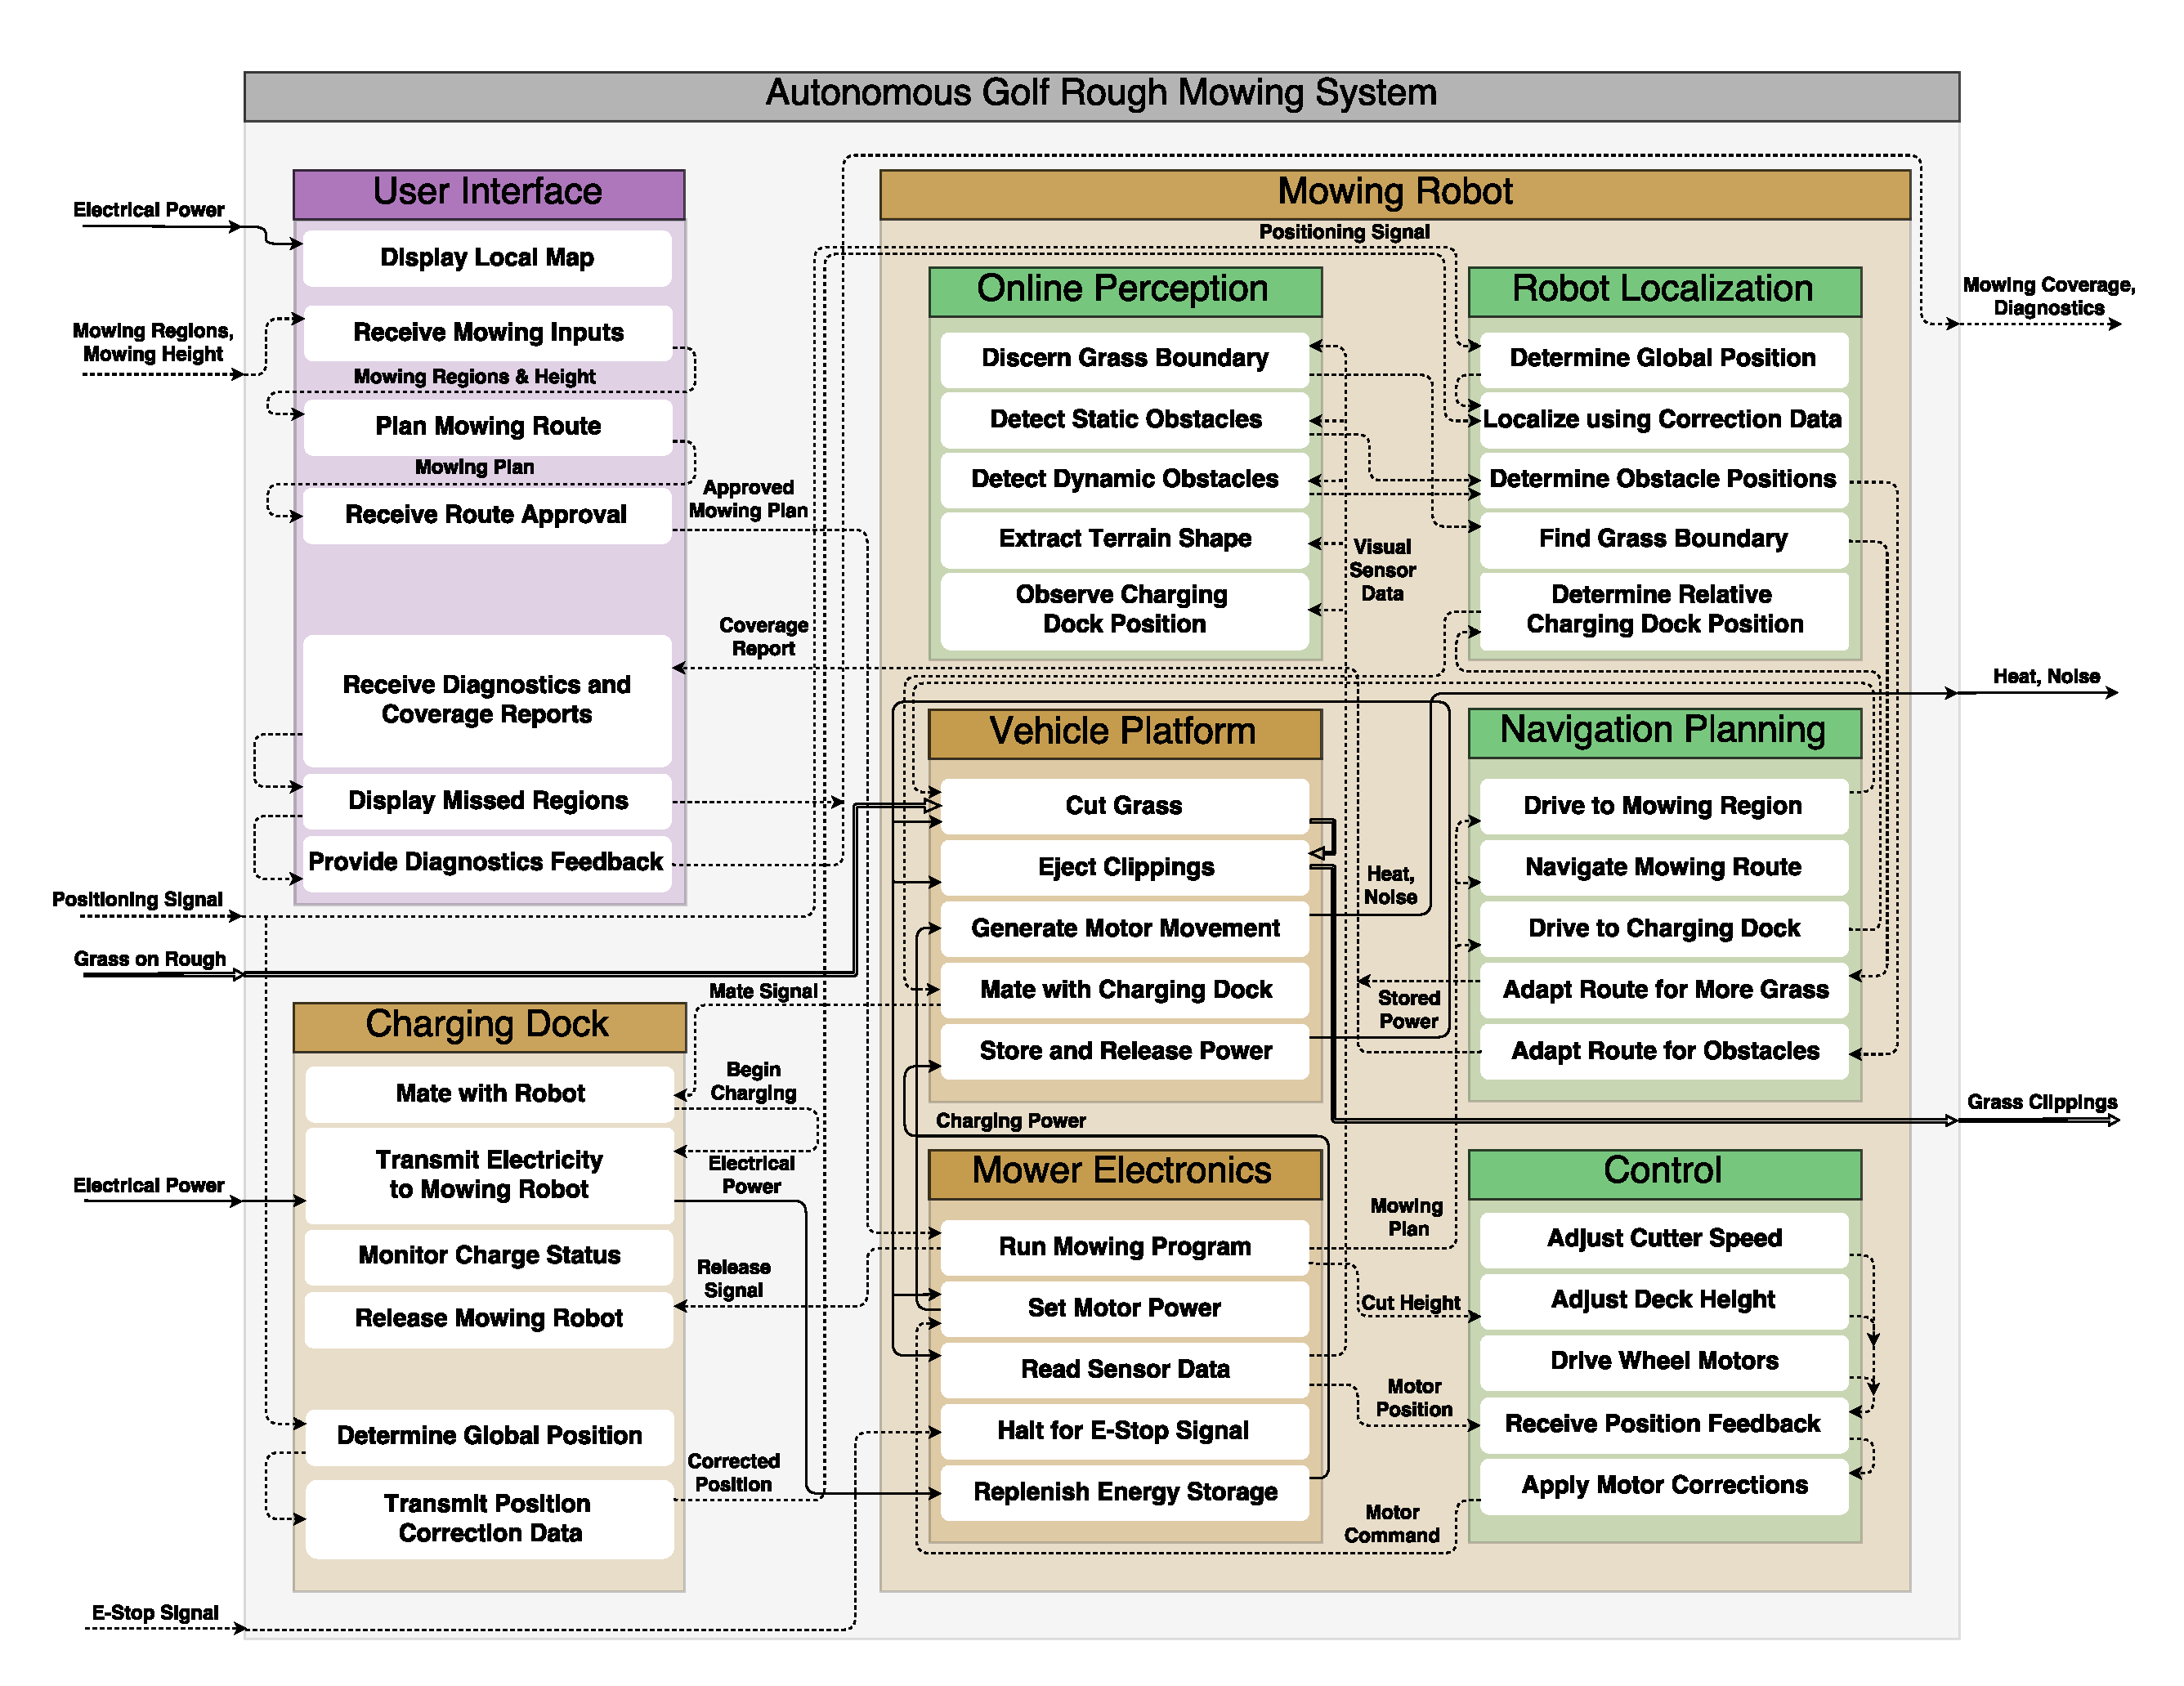
\includegraphics[scale=0.3]{functional}

\section{System Level Trade Studies}

\section{Cyberphysical Architecture}
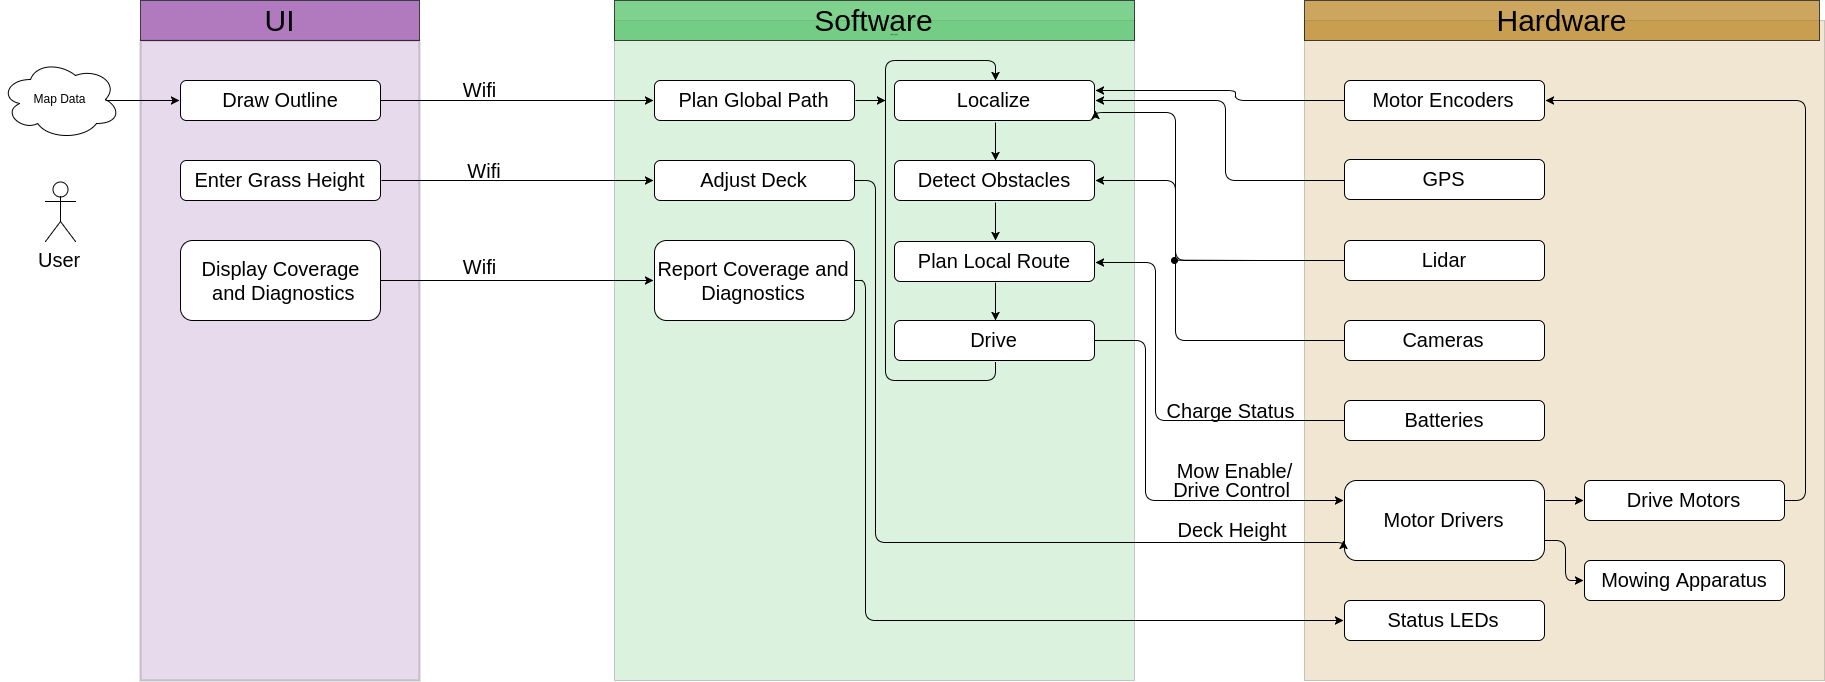
\includegraphics[scale=0.2]{cyberphysical}

\section{Subsystem Descriptions}

\section{Project Management}

\section{References}

\end{document}
